\section*{Task 3a} % (fold)
\label{sec:Task 3a}
	
	\begin{figure}[h]
		\begin{center}
			\newlength\figureheight 
			\newlength\figurewidth 
			\setlength\figureheight{6cm} 
			\setlength\figurewidth{9cm} 
			% This file was created by matlab2tikz v0.2.0.
% Copyright (c) 2008--2012, Nico Schlömer <nico.schloemer@gmail.com>
% All rights reserved.
% 
% 
% 
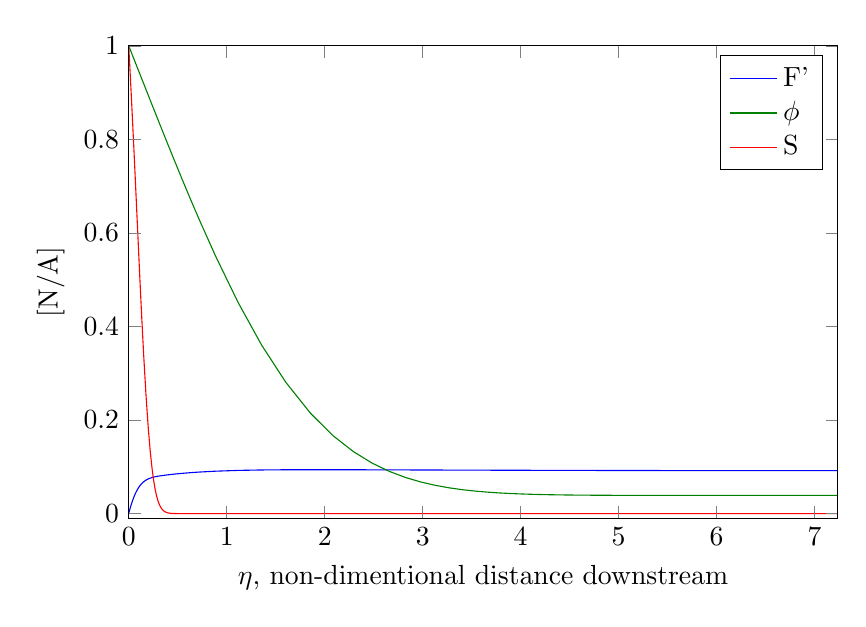
\begin{tikzpicture}

\begin{axis}[%
width=\figurewidth,
height=\figureheight,
scale only axis,
xmin=0, xmax=7.232268737012,
xlabel={$\eta$, non-dimentional distance downstream},
ymin=-0.01, ymax=1,
ylabel={[N/A]},
axis on top,
legend style={nodes=right}]
\addplot [
color=blue,
solid
]
coordinates{
 (0,0)(0.00142151536207323,0.00116653416956551)(0.00852909217243939,0.00681001089873038)(0.02366227352376,0.0178095218684272)(0.0410432016771387,0.0288291429148925)(0.0584280465823158,0.0382583750517365)(0.0751944429660008,0.0459790538649775)(0.0870253046482391,0.0506876282710513)(0.0988561663304774,0.0548402811785791)(0.112159699456503,0.058905579699678)(0.12983893801221,0.0634304941045272)(0.152276694934361,0.0679496308998799)(0.177475992166274,0.071720722020685)(0.200299571052782,0.0742301401777152)(0.220666457260637,0.0759345600970439)(0.238873300370454,0.0771440754324363)(0.25530899284643,0.0780470265413464)(0.27032139418118,0.0787541833252786)(0.284184165031273,0.0793312832657877)(0.297104462004813,0.0798184554341587)(0.309238905372862,0.0802410460034099)(0.320707465374234,0.0806156165295333)(0.331603653331698,0.0809533376906284)(0.342001661835006,0.0812619677633093)(0.351961341043679,0.0815470425161679)(0.361531702386247,0.0818126121574614)(0.37075342451793,0.0820617101217081)(0.379660676772656,0.0822966585553783)(0.388282468885137,0.0825192717846755)(0.396643666254217,0.0827309945609372)(0.40476576518225,0.0829329977337645)(0.412667493087218,0.0831262456072185)(0.420365279193378,0.083311544134307)(0.42787362791949,0.0834895759343099)(0.435205418282192,0.0836609261141848)(0.442372146367658,0.0838261015820298)(0.449384123453311,0.0839855456919073)(0.456250639264069,0.0841396494973528)(0.462980097551305,0.0842887605107307)(0.469580129460632,0.0844331896052112)(0.476057689005694,0.0845732165190222)(0.482419133922059,0.0847090942939108)(0.488670294590823,0.0848410528939596)(0.4948165330539,0.0849693021849899)(0.501118122371576,0.0850992707813553)(0.507875887788803,0.0852369530045107)(0.515170951373743,0.0853836342388603)(0.52311047227652,0.0855410010792832)(0.531837208658068,0.0857112712909797)(0.541547139880878,0.0858974449651891)(0.552519355517513,0.0861037227540903)(0.565169973299464,0.0863362442999506)(0.58015718392977,0.0866044896586391)(0.598607434641521,0.0869241983214461)(0.622673331920724,0.0873242563845964)(0.657209724195049,0.0878660916583559)(0.716723208841552,0.0887157864412036)(0.885511414941763,0.0906255558742339)(1.11559704696663,0.0922917647579597)(1.35657880378265,0.0932363639259047)(1.60324268556716,0.0936745855932849)(1.85567525515445,0.0938023852711316)(2.08434217916761,0.093764558385681)(2.29169549068954,0.0936649089802003)(2.4820284756292,0.0935462588177733)(2.65870784546609,0.0934256486603753)(2.82420902482359,0.0933096874543431)(2.98037103466579,0.0932006720211203)(3.12859153543315,0.0930991008554218)(3.26995750253231,0.0930047418904259)(3.40533202831783,0.092917094887158)(3.53541300941441,0.0928355913548978)(3.66077376479881,0.0927596780576579)(3.78189181414427,0.092688848455865)(3.89916971934952,0.0926226511105586)(4.01295048207048,0.0925606883144474)(4.12352912547211,0.0925026110117608)(4.23116154835446,0.092448112727482)(4.33607139300889,0.0923969236683217)(4.43845544343723,0.0923488054335547)(4.53848791901935,0.0923035464407221)(4.6363239269866,0.0922609580746184)(4.73680153586433,0.0922189455615148)(4.8440950753594,0.0921760135130969)(4.95945231695988,0.0921320786559433)(5.08450939456351,0.0920870522585633)(5.22144996299879,0.0920408527988155)(5.37327889001518,0.0919934251361811)(5.54428895347899,0.0919447837211118)(5.74090804795748,0.0918951134793378)(5.97336331782887,0.0918450214085049)(6.25930422222351,0.0917962306874594)(6.63288076019851,0.0917538066037377)(7.17268776448588,0.0917351701756223)(7.232268737012,0.0917362034568848) 
};

\addlegendentry{F'};

\addplot [
color=green!50!black,
solid
]
coordinates{
 (0,1)(0.00142151536207323,0.999247295315158)(0.00852909217243939,0.995483531382042)(0.02366227352376,0.987468568268171)(0.0410432016771387,0.978261126972536)(0.0584280465823158,0.96904984989953)(0.0751944429660008,0.960165121368419)(0.0870253046482391,0.953895467755127)(0.0988561663304774,0.947625844990646)(0.112159699456503,0.940576195574473)(0.12983893801221,0.931209225092491)(0.152276694934361,0.919324986004269)(0.177475992166274,0.905986140682609)(0.200299571052782,0.893915082615721)(0.220666457260637,0.883153928605581)(0.238873300370454,0.873544278890128)(0.25530899284643,0.864879026255018)(0.27032139418118,0.856973085116734)(0.284184165031273,0.849680899872117)(0.297104462004813,0.842892293886193)(0.309238905372862,0.836523959626854)(0.320707465374234,0.830512071195124)(0.331603653331698,0.824806866366973)(0.342001661835006,0.819368851774819)(0.351961341043679,0.814166158476917)(0.361531702386247,0.80917268014212)(0.37075342451793,0.804366741393812)(0.379660676772656,0.799730128780576)(0.388282468885137,0.795247373442648)(0.396643666254217,0.790905211479829)(0.40476576518225,0.786692171851313)(0.412667493087218,0.782598257277699)(0.420365279193378,0.778614693970611)(0.42787362791949,0.774733733071915)(0.435205418282192,0.770948491414434)(0.442372146367658,0.767252822543876)(0.449384123453311,0.763641211316149)(0.456250639264069,0.760108687030483)(0.462980097551305,0.756650751278571)(0.469580129460632,0.753263317604064)(0.476057689005694,0.749942660678772)(0.482419133922059,0.746685373254216)(0.488670294590823,0.743488329459935)(0.4948165330539,0.740348653372356)(0.501118122371576,0.737133497152385)(0.507875887788803,0.733690026946056)(0.515170951373743,0.729978008766879)(0.52311047227652,0.725944353366645)(0.531837208658068,0.721518460056169)(0.541547139880878,0.716603603115512)(0.552519355517513,0.711062360003955)(0.565169973299464,0.704690404947095)(0.58015718392977,0.697165643970387)(0.598607434641521,0.687939216325888)(0.622673331920724,0.675968382442628)(0.657209724195049,0.658921760513496)(0.716723208841552,0.629939170671103)(0.885511414941763,0.550835471784033)(1.11559704696663,0.451648768917668)(1.35657880378265,0.360131744451815)(1.60324268556716,0.280671293883516)(1.85567525515445,0.214355566654556)(2.08434217916761,0.166683344123815)(2.29169549068954,0.132640900855074)(2.4820284756292,0.108113102038916)(2.65870784546609,0.0902734765329914)(2.82420902482359,0.0771950646724941)(2.98037103466579,0.0675449934053189)(3.12859153543315,0.0603868302992522)(3.26995750253231,0.055053822992063)(3.40533202831783,0.0510660088705673)(3.53541300941441,0.0480747868767)(3.66077376479881,0.0458251018664368)(3.78189181414427,0.0441292040297042)(3.89916971934952,0.0428481821282067)(4.01295048207048,0.0418788149818723)(4.12352912547211,0.0411441182446804)(4.23116154835446,0.0405864924373527)(4.33607139300889,0.0401627222572009)(4.43845544343723,0.0398403056312083)(4.53848791901935,0.0395947454213467)(4.6363239269866,0.0394075427061405)(4.73680153586433,0.039258543243668)(4.8440950753594,0.0391374119332569)(4.95945231695988,0.0390408388463194)(5.08450939456351,0.0389656320735333)(5.22144996299879,0.0389087371450372)(5.37327889001518,0.0388672418749046)(5.54428895347899,0.0388383837105944)(5.74090804795748,0.0388195607447992)(5.97336331782887,0.0388083485256529)(6.25930422222351,0.0388025266616686)(6.63288076019851,0.0388001231233996)(7.17268776448588,0.0387994921340812)(7.232268737012,0.0387994842872832) 
};

\addlegendentry{$\phi$};

\addplot [
color=red,
solid
]
coordinates{
 (0,1)(0.00142151536207323,0.994509651498509)(0.00852909217243939,0.966684380667651)(0.02366227352376,0.905368976892882)(0.0410432016771387,0.831630671412415)(0.0584280465823158,0.754845215843241)(0.0751944429660008,0.678776084604059)(0.0870253046482391,0.624505224868637)(0.0988561663304774,0.570290767474872)(0.112159699456503,0.510048240209998)(0.12983893801221,0.432468372961534)(0.152276694934361,0.340605108607319)(0.177475992166274,0.249685060424384)(0.200299571052782,0.180792801781647)(0.220666457260637,0.130837564754705)(0.238873300370454,0.0951539271972191)(0.25530899284643,0.0696478902534183)(0.27032139418118,0.0512930671235894)(0.284184165031273,0.0379786582685912)(0.297104462004813,0.0282487024734083)(0.309238905372862,0.0210925712084077)(0.320707465374234,0.0158008755339527)(0.331603653331698,0.0118699638900196)(0.342001661835006,0.00893858247524158)(0.351961341043679,0.00674533483612912)(0.361531702386247,0.00509967176785826)(0.37075342451793,0.00386181601816144)(0.379660676772656,0.00292868725868942)(0.388282468885137,0.00222392166421733)(0.396643666254217,0.00169072609153824)(0.40476576518225,0.00128671931972907)(0.412667493087218,0.000980181385702209)(0.420365279193378,0.000747310076044921)(0.42787362791949,0.000570203598893439)(0.435205418282192,0.000435370473866123)(0.442372146367658,0.000332624488991177)(0.449384123453311,0.000254262369102191)(0.456250639264069,0.000194449951800252)(0.462980097551305,0.000148762758514231)(0.469580129460632,0.000113841294611943)(0.476057689005694,8.71318686121273e-05)(0.482419133922059,6.66913350258748e-05)(0.488670294590823,5.10397366803054e-05)(0.4948165330539,3.90489196172431e-05)(0.501118122371576,2.95167114020361e-05)(0.507875887788803,2.17218752811995e-05)(0.515170951373743,1.54694463218233e-05)(0.52311047227652,1.05682255911521e-05)(0.531837208658068,6.83342576438409e-06)(0.541547139880878,4.08710164230114e-06)(0.552519355517513,2.15874262449276e-06)(0.565169973299464,8.86091608691785e-07)(0.58015718392977,1.16324960084668e-07)(0.598607434641521,-2.92156338584956e-07)(0.622673331920724,-4.6683197113769e-07)(0.657209724195049,-5.16068922979271e-07)(0.716723208841552,-5.20293329149578e-07)(0.885511414941763,-5.19726106674707e-07)(1.11559704696663,-5.19664737161256e-07)(1.35657880378265,-5.1964971721224e-07)(1.60324268556716,-5.19646333761501e-07)(1.85567525515445,-5.1964564486923e-07)(2.08434217916761,-5.19645539173328e-07)(2.29169549068954,-5.19645527525922e-07)(2.4820284756292,-5.19645526606411e-07)(2.65870784546609,-5.19645526554971e-07)(2.82420902482359,-5.19645526552989e-07)(2.98037103466579,-5.1964552655294e-07)(3.12859153543315,-5.19645526552939e-07)(3.26995750253231,-5.19645526552939e-07)(3.40533202831783,-5.19645526552939e-07)(3.53541300941441,-5.19645526552939e-07)(3.66077376479881,-5.19645526552939e-07)(3.78189181414427,-5.19645526552939e-07)(3.89916971934952,-5.19645526552939e-07)(4.01295048207048,-5.19645526552939e-07)(4.12352912547211,-5.19645526552939e-07)(4.23116154835446,-5.19645526552939e-07)(4.33607139300889,-5.19645526552939e-07)(4.43845544343723,-5.19645526552939e-07)(4.53848791901935,-5.19645526552939e-07)(4.6363239269866,-5.19645526552939e-07)(4.73680153586433,-5.19645526552939e-07)(4.8440950753594,-5.19645526552939e-07)(4.95945231695988,-5.19645526552939e-07)(5.08450939456351,-5.19645526552939e-07)(5.22144996299879,-5.19645526552939e-07)(5.37327889001518,-5.19645526552939e-07)(5.54428895347899,-5.19645526552939e-07)(5.74090804795748,-5.19645526552939e-07)(5.97336331782887,-5.19645526552939e-07)(6.25930422222351,-5.19645526552939e-07)(6.63288076019851,-5.19645526552939e-07)(7.17268776448588,-5.19645526552939e-07)(7.232268737012,-5.19645526552939e-07) 
};

\addlegendentry{S};

\end{axis}
\end{tikzpicture}

		\end{center}
		\caption{For $T_\infty$ = $2^\circ C$ and $s_\infty$ = $10 \, {}^o/{}_{oo}$ non-dimentionalized velocity, F, temperature, $\phi$, and salinity, $\bar{S}$ versus $\eta$, the non-dimentional distance downstream is presented herein.}
		\label{fig:etaVsF_phi_S_3a}
	\end{figure}
	
	\begin{figure}[h]
		\begin{center}
			\setlength\figureheight{6cm} 
			\setlength\figurewidth{9cm} 
			% This file was created by matlab2tikz v0.2.0.
% Copyright (c) 2008--2012, Nico Schlömer <nico.schloemer@gmail.com>
% All rights reserved.
% 
% 
% 
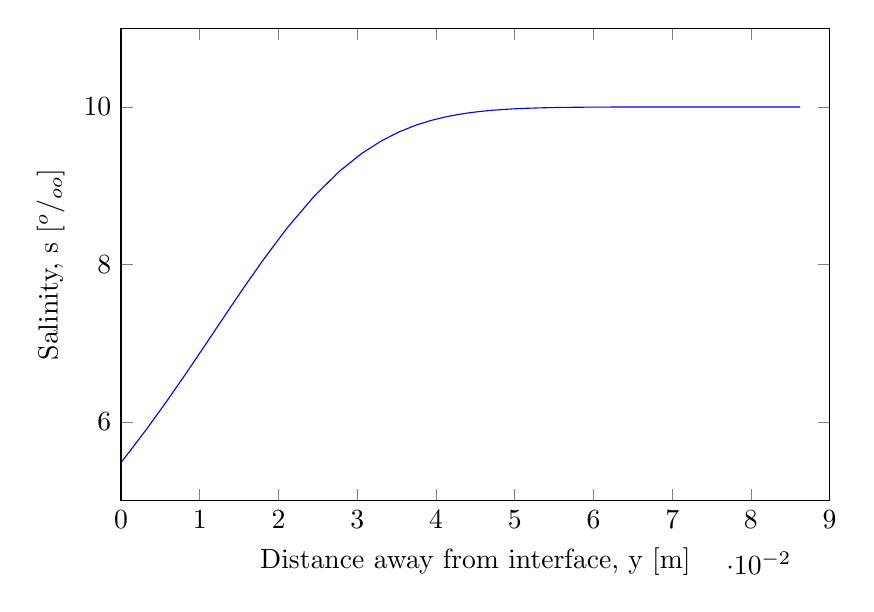
\begin{tikzpicture}

\begin{axis}[%
width=\figurewidth,
height=\figureheight,
scale only axis,
xmin=0, xmax=0.09,
xlabel={Distance away from interface, y [m]},
ymin=5, ymax=11,
ylabel={Salinity, s [${}^o/{}_{oo}$]},
axis on top]
\addplot [
color=blue,
solid
]
coordinates{
 (0,5.48556631203335)(0.000196880873386288,5.51035212626715)(0.00118128524031773,5.63596746628278)(0.00327724145792461,5.91277179067487)(0.005684512182112,6.24565848102947)(0.00809232537916707,6.59230132839681)(0.0104144830227864,6.93571037707733)(0.0120530656530256,7.18071257454183)(0.0136916482832649,7.42546014737508)(0.0155341969400415,7.69742104190788)(0.0179827838639109,8.04765020812232)(0.0210904289147667,8.46236082340958)(0.0245805492329206,8.87281335183817)(0.0277416308960994,9.18382288509506)(0.0305624589024274,9.40934249001984)(0.0330841194266161,9.57043390551855)(0.0353604743473671,9.68557921794416)(0.0374397024480753,9.76844084981813)(0.0393597059213686,9.8285478656885)(0.0411491761025777,9.8724731059127)(0.0428298050089538,9.90477898597093)(0.044418208602609,9.92866799519016)(0.0459273382672494,9.94641383513995)(0.0473674697285257,9.9596473621511)(0.0487468922754554,9.96954863317916)(0.0500723940252213,9.97697786997361)(0.0513496090000658,9.98256608767088)(0.0525832696766728,9.98677863557785)(0.0537773939236204,9.98996025311966)(0.0549354256160665,9.99236732917524)(0.0560603420069444,9.99419119095606)(0.0571547368567629,9.99557503613207)(0.0582208856245901,9.99662631821735)(0.0592607971825839,9.99742585366416)(0.0602762552835702,9.99803454886603)(0.0612688521435372,9.99849838880145)(0.0622400158816304,9.99885214939534)(0.0631910331312584,9.99912216858697)(0.0641230678178729,9.99932842039145)(0.0650371768604867,9.99948607102452)(0.0659343233948608,9.99960664895704)(0.0668153879718248,9.99969892639046)(0.0676811781032442,9.99976958449331)(0.0685324364356805,9.9998237162418)(0.0694052109702984,9.99986674876369)(0.0703411662142452,9.99990193803447)(0.0713515376307853,9.99993016421039)(0.0724511668372735,9.99995229044637)(0.0736598259389982,9.99996915095253)(0.0750046582149431,9.99998154905066)(0.0765243177664043,9.99999025449957)(0.0782764371906741,9.99999599979819)(0.0803521763611713,9.99999947485868)(0.0829075490087295,10.0000013189204)(0.0862406926395122,10.000002107482) 
};

\end{axis}
\end{tikzpicture}

		\end{center}
		\caption{For the same $T_\infty$ and $s_\infty$ as used above, this is the salinity as a function of distance away from the interface.}
		\label{fig:salinity_3a}
	\end{figure}
	
	\begin{figure}[h]
		\begin{center}
			\setlength\figureheight{6cm} 
			\setlength\figurewidth{9cm} 
			% This file was created by matlab2tikz v0.2.0.
% Copyright (c) 2008--2012, Nico Schlömer <nico.schloemer@gmail.com>
% All rights reserved.
% 
% 
% 
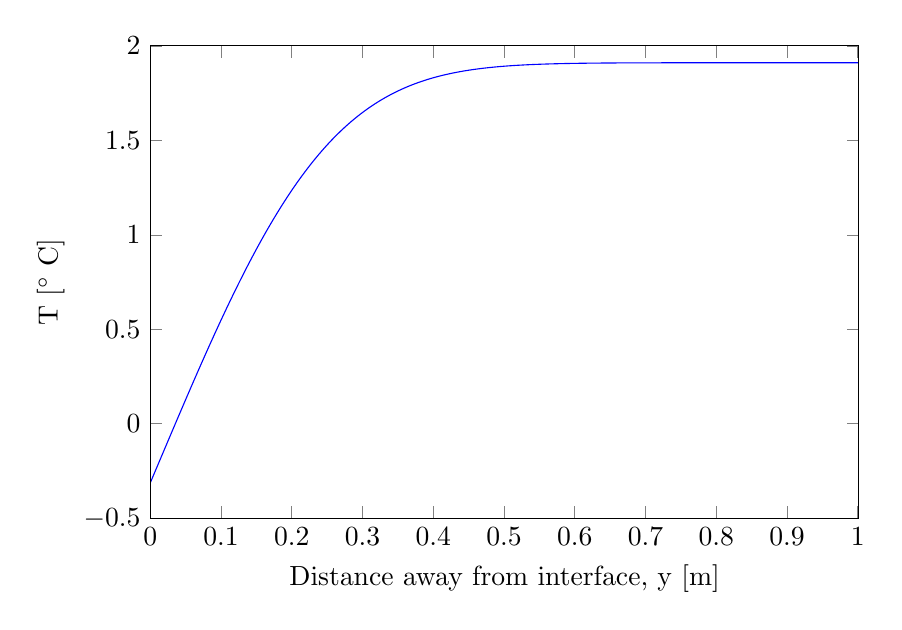
\begin{tikzpicture}

\begin{axis}[%
width=\figurewidth,
height=\figureheight,
scale only axis,
xmin=0, xmax=1.00167428611575,
xlabel={Distance away from interface, y [m]},
ymin=-0.5, ymax=2,
ylabel={T [${}^{\circ}$ C]},
axis on top]
\addplot [
color=blue,
solid
]
coordinates{
 (0,-0.313)(4.24166983427195e-05,-0.312625295932085)(0.000254500190056317,-0.310751749734666)(0.000529373987087325,-0.308323449712033)(0.000878656937926908,-0.305237697508832)(0.00128981601452702,-0.301605149853664)(0.00175390949285143,-0.297504740610367)(0.00226411196440463,-0.292996712518413)(0.00277551776896813,-0.288477812751798)(0.00328662589582211,-0.283961309261244)(0.00379670954325644,-0.279453631751908)(0.00430502249714131,-0.274961383653648)(0.00481079042079197,-0.270491418977175)(0.0053132050289765,-0.266050893666611)(0.00581141745986373,-0.261647324021472)(0.00630453061894389,-0.257288654186888)(0.00679159022140514,-0.252983335131478)(0.00727157415741084,-0.248740418434636)(0.00774337965545046,-0.244569669524908)(0.00820580748643657,-0.240481707067058)(0.00865754208603504,-0.236488178424459)(0.00909712587602814,-0.232601986399413)(0.00952292505104392,-0.22883759142377)(0.00993308228729861,-0.225211429372871)(0.0103254484154465,-0.221742515365664)(0.0106974781715554,-0.218453365167767)(0.0110460597591361,-0.215371501803352)(0.0113672094506014,-0.212532155410766)(0.0116872182302153,-0.209702888681331)(0.0120089696318889,-0.206858212308458)(0.0123325104086052,-0.203997717699146)(0.012657890989729,-0.201120964003322)(0.012985163727177,-0.19822749363259)(0.013317679704687,-0.19528768494851)(0.0136837788716194,-0.192050991480905)(0.0140824089336173,-0.188526733117125)(0.0145129695882453,-0.184720238857409)(0.0149752045211336,-0.180633802810651)(0.0154691477412345,-0.176267159986919)(0.015995091933105,-0.171617767706933)(0.0165535721168103,-0.16668095201817)(0.017145360900145,-0.161449952056116)(0.0177714733766548,-0.155915879678823)(0.0184331808684817,-0.150067601612932)(0.0191320335553435,-0.143891543955113)(0.0198698927562498,-0.137371412533751)(0.0206389102105729,-0.130576732658085)(0.0213884691947083,-0.123954829009907)(0.0221180902258884,-0.117509949452865)(0.0228278457500225,-0.111241455577223)(0.0235180486277546,-0.105146577325659)(0.0241891908072628,-0.0992209567336979)(0.0248418908736659,-0.09345911295916)(0.0254768502542106,-0.0878548305339661)(0.0260948182052515,-0.082401469743052)(0.0266965648633817,-0.0770922055071801)(0.027282861234074,-0.0719202047663945)(0.0278544648525483,-0.0668787535844486)(0.0284121099624441,-0.0619613442111033)(0.0289565011356503,-0.0571617316450661)(0.0294883094861163,-0.0524739672075696)(0.0300081707671132,-0.0478924154232598)(0.0305166848333839,-0.0434117588051635)(0.031014416022424,-0.0390269944923993)(0.0315018941941386,-0.0347334250537354)(0.0319796161519188,-0.030526645908755)(0.0324480473186457,-0.0264025304894813)(0.0329076235222259,-0.0223572144294018)(0.0333587528423976,-0.0183870792095013)(0.0338018174273807,-0.0144887360695782)(0.0342371752613138,-0.010659010354765)(0.0346651618546248,-0.00689492654392065)(0.0350860918513523,-0.00319369401354175)(0.0355002605288028,0.000447306245769719)(0.0359079452060756,0.00403053410544185)(0.0363094065481348,0.00755830185052875)(0.0367048897751843,0.0110327848926781)(0.0370946257826315,0.0144560316911866)(0.0374788321740933,0.0178299729039837)(0.0378577142127478,0.021156429815544)(0.0382314656969061,0.0244371220936992)(0.0386002697667265,0.0276736749365545)(0.0389642996475614,0.0308676256581006)(0.0393237193330263,0.0340204297400379)(0.0396786842136705,0.0371334664017891)(0.0400293416589814,0.0402080437569121)(0.0403758315465968,0.0432454035025309)(0.0407182867585845,0.0462467253162828)(0.0410568336348469,0.0492131308738963)(0.0413915923920568,0.0521456875613977)(0.041722677510653,0.0550454119043866)(0.0420501980923219,0.0579132727358931)(0.0423742581919779,0.0607501941382094)(0.0426949571244196,0.063557058160449)(0.0430123897500633,0.0663347073505898)(0.0433266467362645,0.0690839470716578)(0.0436378148034125,0.0718055476826196)(0.0439459769524624,0.0745002465549491)(0.0442512126762527,0.0771687499455671)(0.0445535981569073,0.0798117347464131)(0.0448532064481592,0.0824298501006018)(0.0451501076476303,0.0850237189293188)(0.0454443690551271,0.0875939393351095)(0.04573605532318,0.0901410859360985)(0.0460252285950125,0.0926657110891878)(0.0463119486359994,0.0951683460552326)(0.0465962729541999,0.0976495020677626)(0.0468782569164101,0.100109671361561)(0.0471579538526957,0.102549328099761)(0.0474354151602436,0.104968929294085)(0.0477106903947595,0.107368915615611)(0.0479838273608708,0.109749712196041)(0.0482548721949249,0.112111729361931)(0.0485238694435944,0.114455363331638)(0.0487908621376506,0.116780996869486)(0.0490558918622397,0.119088999908824)(0.0493189988211915,0.121379730122502)(0.0495802219002061,0.123653533482995)(0.0498395987248165,0.125910744776509)(0.0500971657162245,0.128151688098056)(0.0503529581422916,0.130376677303878)(0.0506070101688346,0.132586016466066)(0.0508593549046447,0.134780000272139)(0.0511100244468661,0.13695891442734)(0.0513590499224095,0.139123036022061)(0.0516064615280339,0.141272633887313)(0.0518522885683302,0.143407968931615)(0.0520965594911931,0.14552929445571)(0.0523393019217916,0.147636856453927)(0.0525805426955724,0.149730893906834)(0.0528203078886076,0.151811639050533)(0.0530586228463883,0.153879317632203)(0.0532955122124146,0.155934149163597)(0.053530999954846,0.157976347157464)(0.0537651093906435,0.160006119341968)(0.053997863210915,0.162023667885315)(0.0542292835030024,0.16402918959191)(0.0544593917728982,0.166022876101159)(0.0546882089660753,0.168004914072314)(0.0549157554872483,0.169975485359878)(0.0551420512195561,0.171934767183801)(0.0553671155426625,0.173882932290147)(0.0555909673502279,0.175820149106132)(0.0558136250668461,0.177746581890377)(0.0560351066638501,0.179662390873222)(0.0562554296742495,0.181567732389371)(0.0564746112077354,0.183462759010986)(0.056692667964586,0.185347619671138)(0.0569096162489359,0.18722245978162)(0.0571254719817925,0.189087421348459)(0.0573402507132001,0.190942643079933)(0.0575539676345081,0.192788260495375)(0.0577666375890309,0.194624406019982)(0.0579782750836701,0.19645120908781)(0.0581888942988917,0.198268796230484)(0.0583985090992404,0.200077291170431)(0.0586071330424362,0.20187681490179)(0.0588147793892961,0.203667485778354)(0.0590214611118426,0.205449419585772)(0.0592271909030383,0.207222729627705)(0.0594319811840302,0.208987526790418)(0.0596358441128248,0.210743919619629)(0.0598387915913914,0.212492014383747)(0.0600408352735979,0.214231915144198)(0.0602419865718697,0.215963723814685)(0.0604422566644192,0.217687540225299)(0.060641656501703,0.219403462179913)(0.0608401968124233,0.221111585509588)(0.0610378881105279,0.222812004134516)(0.0612347407006317,0.224504810112318)(0.061430764683553,0.226190093687276)(0.0616259699621064,0.227867943341722)(0.0618203662464573,0.229538445843596)(0.0620139630594111,0.231201686293395)(0.0622067697411527,0.232857748166356)(0.062398795453901,0.234506713353849)(0.0625900491870785,0.236148662209157)(0.0627805397613454,0.237783673583456)(0.0629702758332752,0.239411824867266)(0.0631592658993072,0.241033192025645)(0.0633475183003287,0.242647849638749)(0.0635350412246109,0.24425587092823)(0.0637218427126992,0.245857327800367)(0.0639079306603999,0.247452290872819)(0.0640933128228067,0.249040829510275)(0.0642779968175526,0.250623011853416)(0.0644619901281654,0.252198904848739)(0.0646453001073077,0.253768574277361)(0.0648279339797467,0.255332084781473)(0.0650098988459428,0.256889499896063)(0.0651912016845623,0.258440882071398)(0.0653718493556156,0.259986292700836)(0.0655518486028391,0.26152579214213)(0.0657312060568672,0.263059439745476)(0.0659099282377644,0.264587293876045)(0.0660880215573726,0.266109411934929)(0.066265492321823,0.267625850381453)(0.0664423467340955,0.269136664755882)(0.0666185908962613,0.270641909699384)(0.0667942308117027,0.272141638973792)(0.066969272387159,0.273635905479842)(0.0671437214354633,0.275124761281305)(0.0673175836769957,0.276608257618124)(0.0674908647419251,0.278086444926275)(0.0676635701723457,0.279559372856703)(0.067838518214424,0.281051070759634)(0.0680158582718969,0.282562797088349)(0.0681956689216646,0.28409520522523)(0.068378032748742,0.285648981718231)(0.0685630366160174,0.287224848501886)(0.0687507719673537,0.288823565394951)(0.0689413351581876,0.290445932823924)(0.0691348278178695,0.292092794807608)(0.0693313572441504,0.293765042205035)(0.069531036837088,0.295463616287401)(0.0697339865748473,0.297189512653607)(0.069940333536572,0.29894378553182)(0.0701502124793643,0.300727552525009)(0.0703637664745241,0.302541999842086)(0.0705811476119318,0.304388388087697)(0.0708025177802698,0.306268058673189)(0.071028049534781,0.308182440944805)(0.0712579270627936,0.310133060112148)(0.0714923472613802,0.312121546094426)(0.0717315209440984,0.314149643423083)(0.0719756741938741,0.316219222339455)(0.0722250498856794,0.318332291280861)(0.0724799094041061,0.320491010959448)(0.0727405345875052,0.32269771029215)(0.0730072299346224,0.324954904474169)(0.073280325117717,0.327265315554205)(0.0735601778560408,0.329631895950316)(0.0738471772109709,0.332057855404304)(0.0741417473825879,0.334546692024375)(0.0744443520989342,0.337102228156685)(0.0747554997165744,0.339728652050515)(0.0750757491703169,0.342430566434997)(0.075405716951956,0.345213045468064)(0.0757460853398266,0.348081701856749)(0.0760976121517305,0.351042766356315)(0.0764611423823605,0.354103182576292)(0.0768376221690542,0.357270720683792)(0.0772281156790053,0.360554114805655)(0.0776338256734285,0.363963230235154)(0.0780561187558334,0.367509268580677)(0.0784965566468054,0.371205021693852)(0.0789569352903559,0.375065188935639)(0.0794393342701514,0.379106777754691)(0.079946179965634,0.383349615194004)(0.0804803272960272,0.387817009323741)(0.0810451670007535,0.392536616432758)(0.0816447686362399,0.39754159568739)(0.082284074508672,0.402872173263449)(0.0829691678747898,0.408577802743456)(0.0837076521568122,0.414720215528261)(0.084509200897696,0.421377837948008)(0.0853863790400496,0.42865237639414)(0.0863559121022653,0.436678974329148)(0.087440728639308,0.445642522159729)(0.0886734112794661,0.455805145477873)(0.0901023866149864,0.467555361017342)(0.091803891661503,0.481502758678945)(0.0939074639662832,0.498678751774656)(0.0966578330633513,0.521020987199192)(0.100596296317811,0.552780118935325)(0.106908766815444,0.60307997489803)(0.1132476459124,0.652803971434301)(0.119534190110329,0.701295409048041)(0.125766463723352,0.748519483641724)(0.131944941142117,0.794464434243139)(0.138069905287865,0.839120954782643)(0.144141333487338,0.882481365639911)(0.150158871680497,0.924539496067008)(0.156121806935516,0.965290578092564)(0.162029034328532,1.00473112624568)(0.167879017221098,1.04285880104435)(0.173669740309419,1.07967225709303)(0.179398653495853,1.11517096871557)(0.185062606409921,1.14935503831351)(0.190657770209196,1.18222497327291)(0.196179545781853,1.21378143422519)(0.201626738649131,1.24404840716219)(0.207237978837748,1.27432752610981)(0.213031402105662,1.3046308523974)(0.219024049451691,1.33495189598028)(0.22523552635837,1.36528374677338)(0.231688655412034,1.39561948820044)(0.238410268216696,1.4259524000373)(0.245018335906828,1.45452705049057)(0.251485680085723,1.48131159041655)(0.257819188581416,1.50642487623284)(0.264025938088396,1.52998007085677)(0.270112489086833,1.55208199393929)(0.27608491415568,1.57282770681711)(0.281948839542696,1.59230712562656)(0.28770948394595,1.61060359244191)(0.293371694021011,1.62779440240759)(0.298939976781588,1.64395128839954)(0.304418529021913,1.6591408652498)(0.309811263999091,1.67342503625975)(0.315121835544138,1.68686136467707)(0.320353659885146,1.69950341314767)(0.325509935412336,1.71140105390732)(0.330593660511904,1.72260075212821)(0.335607649701939,1.73314582497086)(0.340554548281565,1.74307667865019)(0.345436845560238,1.75243102536566)(0.350256886894723,1.76124408214013)(0.355016884596952,1.76954875311995)(0.359718927856149,1.77737579692248)(0.364364991790295,1.78475398042248)(0.368956945654238,1.79171022011275)(0.37349656037158,1.79826971229895)(0.377985515402453,1.80445605303235)(0.382425405025093,1.81029134871285)(0.386817744094554,1.81579631818846)(0.391163973311288,1.82099038706567)(0.395465464093856,1.82589177495692)(0.399723523026771,1.83051757618001)(0.4039393959688,1.83488383451744)(0.40811427184616,1.83900561251603)(0.412249286144787,1.84289705575899)(0.416345524139993,1.84657145253028)(0.420404023887279,1.85004128924012)(0.424425778999729,1.85331830194988)(0.428411741202667,1.8564135242794)(0.432362822725146,1.85933733201185)(0.436279898512787,1.86209948462433)(0.440163808296997,1.8647091639933)(0.444015358498075,1.86717501046345)(0.447835324028637,1.86950515651321)(0.451624449952416,1.87170725815777)(0.455383453052304,1.87378852428288)(0.45911302328418,1.87575574404001)(0.462813825136679,1.87761531244977)(0.466486498912994,1.87937325434553)(0.470131661923036,1.88103524676515)(0.473749909614385,1.88260663991013)(0.477341816617587,1.88409247675847)(0.480907937738339,1.88549751143623)(0.484448808896649,1.88682622643035)(0.487964947994988,1.88808284871284)(0.49145685574655,1.88927136486079)(0.494925016453457,1.89039553523386)(0.498369898740153,1.89145890727303)(0.501791956246325,1.89246482797921)(0.505191628283512,1.89341645562585)(0.508569340451257,1.89431677075392)(0.511925505222538,1.89516858649793)(0.515260522492085,1.89597455828411)(0.518574780110001,1.896737192946)(0.52186865437233,1.89745885728733)(0.52514251049334,1.89814178613306)(0.528396703050711,1.89878808989842)(0.531631576413092,1.89939976170801)(0.534847465136141,1.89997868409025)(0.538044694353741,1.90052663527835)(0.541223580135165,1.90104529513672)(0.54438442983455,1.90153625074059)(0.547527542421742,1.9020010016279)(0.550653208789962,1.90244096474302)(0.553761712062204,1.90285747909403)(0.556853327869021,1.90325181013719)(0.559928324627734,1.90362515390887)(0.562986963796443,1.90397864091685)(0.566029500124022,1.90431333980795)(0.569056181883801,1.9046302608239)(0.572067251106245,1.90493035905973)(0.575062943783227,1.90521453753346)(0.578043490086429,1.90548365008274)(0.581009114559721,1.90573850409437)(0.583960036306034,1.90597986307887)(0.58689646917326,1.9062084490993)(0.589818621922364,1.90642494506157)(0.592726698401792,1.90662999687604)(0.595620897695265,1.90682421549579)(0.598501414286786,1.90700817884146)(0.601368438198864,1.90718243361644)(0.604222155135797,1.90734749702086)(0.607062746617251,1.90750385836913)(0.609890390111371,1.90765198061722)(0.612705259157292,1.90779230180434)(0.615507523485286,1.90792523641418)(0.618297349130205,1.90805117666032)(0.621074898545167,1.90817049370032)(0.623840330707329,1.90828353878216)(0.626593801218026,1.90839064432711)(0.629373821323339,1.90849350957099)(0.632188711226069,1.90859250841575)(0.635039631282287,1.90868772643861)(0.637927796463435,1.90877924846232)(0.640854484027847,1.90886715869396)(0.643821037905846,1.90895154072535)(0.646828873485957,1.90903247753355)(0.649879482841525,1.90911005148121)(0.652974440430736,1.9091843443165)(0.656115409359799,1.9092554371733)(0.659304148242046,1.90932341057099)(0.662542518735402,1.90938834441409)(0.665832493848014,1.90945031799182)(0.66917616710598,1.90950940997765)(0.672575762673964,1.90956569842833)(0.676033646576038,1.90961926078297)(0.679552339147388,1.90967017386187)(0.683134528893574,1.9097185138652)(0.686783087941143,1.90976435637132)(0.690501089324768,1.90980777633515)(0.694291826344185,1.90984884808595)(0.698158834341336,1.90988764532516)(0.702105915222866,1.90992424112369)(0.706137165210733,1.9099587079192)(0.710257006285692,1.90999111751284)(0.714470221972383,1.91002154106577)(0.718781998188882,1.91005004909522)(0.723197970059437,1.91007671147034)(0.727724275754625,1.91010159740744)(0.732367618667431,1.91012477546484)(0.737135339533904,1.91014631353723)(0.74203550046887,1.91016627884948)(0.747076983350285,1.91018473794976)(0.752269605611468,1.91020175670213)(0.757624257285042,1.91021740027826)(0.763153064111218,1.91023173314838)(0.768869582967787,1.91024481907133)(0.774789037556267,1.91025672108349)(0.780928604747315,1.91026750148661)(0.787307765261641,1.91027722183424)(0.793948736762727,1.91028594291666)(0.800877013802482,1.91029372474403)(0.8081220477914,1.9103006265275)(0.815718112888542,1.91030670665788)(0.823705422230238,1.91031202268145)(0.832131586419283,1.91031663127246)(0.84105354797367,1.91032058820134)(0.850540190550878,1.91032394829803)(0.860675925061955,1.91032676540892)(0.871565724889129,1.91032909234598)(0.883342369896201,1.91033098082556)(0.896177164747106,1.91033248139388)(0.910296324618008,1.91033364333438)(0.926007008731381,1.91033451454988)(0.94374063417383,1.91033514140869)(0.964129103953622,1.91033556853642)(0.98814868489841,1.91033583852286)(1.00167428611575,1.91033592413086) 
};

\end{axis}
\end{tikzpicture}

		\end{center}
		\caption{Temperature in the water as a function of distance away from the interface.}
		\label{fig:temperture_3a}
	\end{figure}
	
	\begin{figure}[h]
		\begin{center}
			\setlength\figureheight{6cm} 
			\setlength\figurewidth{9cm} 
			% This file was created by matlab2tikz v0.2.0.
% Copyright (c) 2008--2012, Nico Schlömer <nico.schloemer@gmail.com>
% All rights reserved.
% 
% 
% 
\begin{tikzpicture}

\begin{axis}[%
width=\figurewidth,
height=\figureheight,
scale only axis,
xmin=0, xmax=1.4,
xlabel={Distance away from interface, y [m]},
ymin=0, ymax=6,
ylabel={u [mm/s]},
axis on top]
\addplot [
color=blue,
solid
]
coordinates{
 (0,0)(0.000196880873386288,0.0708035982738613)(0.00118128524031773,0.413338321751788)(0.00327724145792461,1.08096124804585)(0.005684512182112,1.74980476935884)(0.00809232537916707,2.32211853578435)(0.0104144830227864,2.79073047648544)(0.0120530656530256,3.07652065682316)(0.0136916482832649,3.3285687972946)(0.0155341969400415,3.57531490286167)(0.0179827838639109,3.84995771239367)(0.0210904289147667,4.1242498459211)(0.0245805492329206,4.35313882983407)(0.0277416308960994,4.50544970055437)(0.0305624589024274,4.60890064644742)(0.0330841194266161,4.68231301630976)(0.0353604743473671,4.73711825840569)(0.0374397024480753,4.78003962852279)(0.0393597059213686,4.81506710857243)(0.0411491761025777,4.84463636029215)(0.0428298050089538,4.87028578718441)(0.044418208602609,4.89302060434518)(0.0459273382672494,4.91351882380811)(0.0473674697285257,4.93225133953843)(0.0487468922754554,4.9495541488397)(0.0500723940252213,4.96567308190352)(0.0513496090000658,4.98079225513608)(0.0525832696766728,4.99505261282355)(0.0537773939236204,5.00856427674975)(0.0549354256160665,5.02141493709641)(0.0560603420069444,5.0336756593899)(0.0571547368567629,5.04540497273219)(0.0582208856245901,5.05665179499853)(0.0592607971825839,5.06745755823825)(0.0602762552835702,5.07785777592286)(0.0612688521435372,5.08788321518998)(0.0622400158816304,5.09756078572107)(0.0631910331312584,5.10691422278096)(0.0641230678178729,5.11596461887295)(0.0650371768604867,5.12473084265915)(0.0659343233948608,5.13322987304477)(0.0668153879718248,5.14147706857368)(0.0676811781032442,5.14948638707493)(0.0685324364356805,5.15727056649969)(0.0694052109702984,5.16515910035095)(0.0703411662142452,5.17351581811549)(0.0713515376307853,5.18241873708877)(0.0724511668372735,5.19197022631354)(0.0736598259389982,5.20230489458258)(0.0750046582149431,5.21360483450873)(0.0765243177664043,5.22612500758143)(0.0782764371906741,5.24023806363468)(0.0803521763611713,5.25651940121649)(0.0829075490087295,5.27592433963719)(0.0862406926395122,5.30020614048667)(0.0910240071614626,5.33309320719657)(0.0992666664728442,5.38466601974655)(0.122643951250019,5.50058079640701)(0.154510972455209,5.60171249706487)(0.187887114576462,5.65904559691046)(0.22205023498605,5.68564376411515)(0.257012322697157,5.69340065395676)(0.288682851848954,5.69110472498076)(0.317401430741016,5.685056435391)(0.34376268247908,5.6778548817162)(0.368232898961365,5.67053436479098)(0.391154928232187,5.66349601918443)(0.412783475983264,5.6568792520627)(0.433312119164629,5.6507143199073)(0.452891404631505,5.64498713726198)(0.471640871279573,5.63966734177618)(0.489657178280215,5.63472042851242)(0.507019730713308,5.63011281842979)(0.52379466538809,5.62581376675854)(0.54003773740952,5.62179587309871)(0.555796452747207,5.61803499833118)(0.571111672316154,5.61450995627452)(0.586018838279421,5.6112021452156)(0.600548925251017,5.60809518986413)(0.61472918795304,5.6051746203232)(0.628583755891634,5.60242759444912)(0.642134111526994,5.59984266411153)(0.656050330738838,5.59729268557007)(0.670910561115586,5.59468689519671)(0.686887619882375,5.59202023865352)(0.704208112730113,5.58928733032132)(0.723174477382149,5.58648322215733)(0.744202890126626,5.58360456736962)(0.767887903705019,5.58065224303837)(0.795119786017488,5.57763747335869)(0.8273150037243,5.5745971004725)(0.866918019278052,5.57163571391176)(0.918658631469448,5.56906075480697)(0.993422279685765,5.56792960391232)(1.00167428611575,5.56799231963323) 
};

\end{axis}
\end{tikzpicture}

		\end{center}
		\caption{Velocity in the water as a function of distance away from the interface.}
		\label{fig:salinity_3a}
	\end{figure}
	
	\begin{figure}[h]
		\begin{center}
			\setlength\figureheight{6cm} 
			\setlength\figurewidth{9cm} 
			% This file was created by matlab2tikz v0.2.0.
% Copyright (c) 2008--2012, Nico Schlömer <nico.schloemer@gmail.com>
% All rights reserved.
% 
% 
% 
\begin{tikzpicture}

\begin{axis}[%
width=\figurewidth,
height=\figureheight,
scale only axis,
xmin=0, xmax=1,
xlabel={x, Height of ice [m]},
ymin=4, ymax=18,
ylabel={h [$W/m^2 K$]},
axis on top]
\addplot [
color=blue,
solid
]
coordinates{
 (0.0101010101010101,16.0223860476003)(0.0202020202020202,13.4731669912382)(0.0303030303030303,12.1743806882529)(0.0404040404040404,11.3295378250469)(0.0505050505050505,10.7148153319222)(0.0606060606060606,10.2373930786859)(0.0707070707070707,9.85037312407628)(0.0808080808080808,9.52696774356328)(0.0909090909090909,9.25052889764212)(0.101010101010101,9.01004980271889)(0.111111111111111,8.7978999780521)(0.121212121212121,8.60858714141014)(0.131313131313131,8.43803560235741)(0.141414141414141,8.28314344894727)(0.151515151515152,8.14149905436128)(0.161616161616162,8.01119302380013)(0.171717171717172,7.89068962777785)(0.181818181818182,7.77873658922815)(0.191919191919192,7.67430033347565)(0.202020202020202,7.57651858036375)(0.212121212121212,7.48466501665652)(0.222222222222222,7.39812255330474)(0.232323232323232,7.31636279360572)(0.242424242424242,7.23893006761101)(0.252525252525253,7.16542887283567)(0.262626262626263,7.09551388980557)(0.272727272727273,7.02888196757977)(0.282828282828283,6.96526563325205)(0.292929292929293,6.90442779247699)(0.303030303030303,6.8461573696039)(0.313131313131313,6.79026569555817)(0.323232323232323,6.7365834956191)(0.333333333333333,6.68495836211735)(0.343434343434343,6.63525262187806)(0.353535353535354,6.58734152712632)(0.363636363636364,6.54111171308486)(0.373737373737374,6.49645987673648)(0.383838383838384,6.45329164000006)(0.393939393939394,6.41152056746979)(0.404040404040404,6.37106731433104)(0.414141414141414,6.33185888441955)(0.424242424242424,6.29382798188135)(0.434343434343434,6.25691244270521)(0.444444444444444,6.22105473468162)(0.454545454545455,6.18620151620239)(0.464646464646465,6.1523032458387)(0.474747474747475,6.11931383588915)(0.484848484848485,6.08719034412643)(0.494949494949495,6.05589269883163)(0.505050505050505,6.02538345292298)(0.515151515151515,5.99562756358649)(0.525252525252525,5.96659219432044)(0.535353535353535,5.93824653673141)(0.545454545454545,5.9105616497793)(0.555555555555556,5.88351031447462)(0.565656565656566,5.85706690229154)(0.575757575757576,5.83120725578271)(0.585858585858586,5.80590858007202)(0.595959595959596,5.78114934406569)(0.606060606060606,5.75690919036272)(0.616161616161616,5.73316885296779)(0.626262626262626,5.70991008201513)(0.636363636363636,5.68711557480369)(0.646464646464647,5.66476891252344)(0.656565656565657,5.6428545021224)(0.666666666666667,5.62135752282482)(0.676767676767677,5.60026387686395)(0.686868686868687,5.57956014404007)(0.696969696969697,5.5592335397552)(0.707070707070707,5.53927187621245)(0.717171717171717,5.51966352649987)(0.727272727272727,5.50039739130714)(0.737373737373737,5.48146286804845)(0.747474747474748,5.4628498221873)(0.757575757575758,5.44454856057881)(0.767676767676768,5.42654980666281)(0.777777777777778,5.40884467735662)(0.787878787878788,5.39142466151081)(0.797979797979798,5.37428159980362)(0.808080808080808,5.35740766596108)(0.818181818181818,5.34079534920009)(0.828282828282828,5.32443743780078)(0.838383838383838,5.30832700372284)(0.848484848484849,5.29245738818755)(0.858585858585859,5.27682218815445)(0.868686868686869,5.26141524362717)(0.878787878787879,5.24623062572867)(0.888888888888889,5.23126262549092)(0.898989898989899,5.2165057433088)(0.909090909090909,5.20195467901169)(0.919191919191919,5.18760432251032)(0.929292929292929,5.17344974497956)(0.939393939393939,5.15948619054093)(0.94949494949495,5.14570906841164)(0.95959595959596,5.13211394548916)(0.96969696969697,5.11869653934294)(0.97979797979798,5.10545271158695)(0.98989898989899,5.09237846160866)(1,5.07946992063178) 
};

\end{axis}
\end{tikzpicture}

		\end{center}
		\caption{Heat transfer coefficient along the ice water interface.}
		\label{fig:temperture_3a}
	\end{figure}
	
	\begin{figure}[h]
		\begin{center}
			\setlength\figureheight{6cm} 
			\setlength\figurewidth{9cm} 
			% This file was created by matlab2tikz v0.2.0.
% Copyright (c) 2008--2012, Nico Schlömer <nico.schloemer@gmail.com>
% All rights reserved.
% 
% 
% 
\begin{tikzpicture}

\begin{axis}[%
width=\figurewidth,
height=\figureheight,
scale only axis,
xmin=0, xmax=2,
xlabel={$T_\infty [^{\circ}C]$ },
ymin=1, ymax=7,
ylabel={$h [W/m^2/s]$},
axis on top]
\addplot [
color=blue,
solid,
mark=square,
mark options={solid}
]
coordinates{
 (0,1.1565873919785)(1,3.99816088148382)(2,6.8743773691225) 
};

\end{axis}
\end{tikzpicture}

		\end{center}
		\caption{Mean heat transfer coefficient over $\unit[1]{m}$ long section of ice as a function of ambient temperature.}
		\label{fig:h_Tinf}
	\end{figure}
	
	\begin{figure}[h]
		\begin{center}
			\setlength\figureheight{6cm} 
			\setlength\figurewidth{9cm} 
			% This file was created by matlab2tikz v0.2.0.
% Copyright (c) 2008--2012, Nico Schlömer <nico.schloemer@gmail.com>
% All rights reserved.
% 
% 
% 
\begin{tikzpicture}

\begin{axis}[%
width=\figurewidth,
height=\figureheight,
scale only axis,
xmin=0, xmax=2,
xlabel={$T_\infty$ },
ymin=1, ymax=7,
ylabel={$\dot{M}$ [cm/day]},
axis on top]
\addplot [
color=blue,
solid,
mark=square,
mark options={solid}
]
coordinates{
 (0,1.03209220509675)(1,3.56779842934594)(2,6.13441867581481) 
};

\end{axis}
\end{tikzpicture}

		\end{center}
		\caption{Mean ice melting rate over a $\unit[1]{m}$ long section of ice as a function of ambient temperature.}
		\label{fig:Mdot_Tinf}
	\end{figure}

	\begin{figure}[h]
		\begin{center}
			\setlength\figureheight{6cm} 
			\setlength\figurewidth{9cm} 
			% This file was created by matlab2tikz v0.2.0.
% Copyright (c) 2008--2012, Nico Schlömer <nico.schloemer@gmail.com>
% All rights reserved.
% 
% 
% 
\begin{tikzpicture}

\begin{axis}[%
width=\figurewidth,
height=\figureheight,
scale only axis,
xmin=10, xmax=20,
xlabel={$s_\infty$ },
ymin=1.1, ymax=2.1,
ylabel={$h [W/m^2/s]$},
axis on top]
\addplot [
color=blue,
solid,
mark=square,
mark options={solid}
]
coordinates{
 (10,1.1565873919785)(20,2.07438020996298) 
};

\end{axis}
\end{tikzpicture}

		\end{center}
		\caption{Mean heat transfer coefficient over $\unit[1]{m}$ long section of ice as a function of ambient salinity.}
		\label{fig:h_sinf}
	\end{figure}

	\begin{figure}[h]
		\begin{center}
			\setlength\figureheight{6cm} 
			\setlength\figurewidth{9cm} 
			% This file was created by matlab2tikz v0.2.0.
% Copyright (c) 2008--2012, Nico Schlömer <nico.schloemer@gmail.com>
% All rights reserved.
% 
% 
% 
\begin{tikzpicture}

\begin{axis}[%
width=\figurewidth,
height=\figureheight,
scale only axis,
xmin=10, xmax=20,
xlabel={$s_\infty$ },
ymin=2.15, ymax=2.18,
ylabel={$\dot{M}$ [cm/day]},
axis on top]
\addplot [
color=blue,
solid,
mark=square,
mark options={solid}
]
coordinates{
 (10,2.1781170208897)(20,2.15042586219733) 
};

\end{axis}
\end{tikzpicture}

		\end{center}
		\caption{Mean ice melting rate over a $\unit[1]{m}$ long section of ice as a function of ambient salinity.}
		\label{fig:Mdot_sinf}
	\end{figure}


	Ice melting rate can be related to the injection velocity of fresh water $v_0$, by taking into account the expansion of water as it melts. This gives
	\begin{equation*}
	  v_1 = \frac{\rho_l}{\rho_i}(1-s_0/1000)v_0
	\end{equation*}

	By taking the average of the ice melting rate over a $\unit[1]{m}$ long surface the numbers in figure~\ref{something} are generated.

	\begin{table}
	  \centering
	  \begin{tabular}{lllll}
	    $T_\infty [\unit{^\circ C}]$ & $s_\infty [\permil]$ & $\text{CGr} [\unit{m^{-3}}]$ & $h_{av} [\unit{W/m^2/K}]$ & $\dot{M}_{av} [\unit{cm/day}]$ \\
	    \hline
	    $0$ & $10$ & $2912$ & $1.157$ & $32.64$ \\
	    $1$ & $10$ & $7341$ & $3.998$ & $112.8$ \\
	    $2$ & $10$ & $10870$ & $6.874$ & $194.0$ \\
	    $0$ & $20$ & $8192$ & $2.074$ & $58.54$ \\
	  \end{tabular}
	  \caption{<+Caption text+>}
	  \label{tab:<+label+>}
	\end{table}<++>

% section Task 3a (end)
